\documentclass{computacion}
\titulo{Hallazgos de la prueba de despliegue desde cero}
\tipo{Proyecto Tecnológico}
\version{Bitácora de instalación}
\trimestre{2026-Primavera}
\alumno{[TU NOMBRE]}
\matricula{[MATRÍCULA]}

\asesor{[Grado. Nombres Apellidos del Asesor]}
\categoria{[Profesor Titular/Asociado/Asistente]}
\departamento{[Departamento de Sistemas]}
\correo{[correo@azc.uam.mx]}

\coasesor{}
\categoriacoasesor{}
\departamentocoasesor{}
\correocoasesor{}

\usepackage{float}

\begin{document}
\portada
\setcounter{page}{1}
\pagestyle{fancy}

\section{Contexto de la prueba}

Este documento acompaña al \emph{Manual de Instalación} (\texttt{main.pdf}) como bitácora de una prueba de despliegue \emph{desde cero} realizada sobre una copia limpia del repositorio. Documenta la reproducibilidad completa del sistema —incluyendo el nuevo \emph{script de bootstrap unificado}— y deja registrada la trazabilidad de los ajustes de código y documentación que fueron necesarios para llegar al estado actual.

\begin{longtable}{p{0.30\textwidth} p{0.62\textwidth}}
    \toprule
    \textbf{Elemento} & \textbf{Valor} \\
    \midrule
    \endhead
    Fecha de la prueba          & 2026-08-21 \\
    Repositorio                 & \url{https://github.com/Aldebaran-GR/proyecto_terminal_cyad.git} \\
    Commit probado              & \texttt{a2b8123} (H7, H8 y bootstrap unificados) \\
    Sistema operativo           & Windows 11 Home 10.0.26200 \\
    Shells utilizados           & PowerShell 5.1 y Git Bash 2.47 \\
    Modalidad                   & Clon fresco en carpeta paralela \\
    Base de datos               & PostgreSQL 17, base \texttt{proyecto\_terminal\_cyad\_test} (aislada) \\
    Bootstrap                   & \texttt{scripts/bootstrap.ps1} — 9.8\,s end-to-end \\
    \bottomrule
\end{longtable}

\section{Prerrequisitos verificados}

\begin{Verbatim}[fontsize=\small, frame=single]
$ python --version           → Python 3.13.0
$ node --version             → v22.16.0
$ npm --version              → 10.9.2
$ git --version              → git version 2.47.0.windows.2
$ psql --version             → psql (PostgreSQL) 17.0
\end{Verbatim}

Todos los prerrequisitos del manual están cubiertos por versiones iguales o superiores.

\section{Rutas utilizadas}

\begin{longtable}{p{0.28\textwidth} p{0.64\textwidth}}
    \toprule
    \textbf{Recurso} & \textbf{Ruta} \\
    \midrule
    \endhead
    Carpeta padre de la prueba & \texttt{C:\textbackslash Users\textbackslash godin\textbackslash Documents\textbackslash 10\_2025\_Proyectos\textbackslash prueba\_despliegue\textbackslash} \\
    Clon del repositorio       & \texttt{prueba\_despliegue\textbackslash proyecto\_terminal\_cyad\textbackslash} \\
    Script de bootstrap        & \texttt{scripts\textbackslash bootstrap.ps1} \\
    Entorno virtual Python     & \texttt{...\textbackslash backend\textbackslash .venv\textbackslash} \\
    Archivo \texttt{.env}      & \texttt{...\textbackslash backend\textbackslash .env} \\
    Backend (dev server)       & \url{http://localhost:8000} \\
    OpenAPI Swagger UI         & \url{http://localhost:8000/api/docs/} \\
    Frontend (Vite dev)        & \url{http://localhost:5173} \\
    \bottomrule
\end{longtable}

\section{Cronología por fase}

\begin{longtable}{p{0.10\textwidth} p{0.42\textwidth} p{0.15\textwidth} p{0.25\textwidth}}
    \toprule
    \textbf{Fase} & \textbf{Comando principal} & \textbf{Duración} & \textbf{Resultado} \\
    \midrule
    \endhead
    A & Verificación de prerrequisitos             & --      & OK (5/5) \\
    B & \texttt{git clone --depth 1}               & 0.9\,s  & OK (17 MB) \\
    C & \texttt{python -m venv .venv}              & \textless\,3\,s & OK \\
    C & \texttt{pip install -r requirements.txt}   & 46.1\,s & OK, 28 paquetes \\
    C & \texttt{scripts/bootstrap.ps1}             & \textbf{9.8\,s}  & OK end-to-end (crea BD + migra + siembra) \\
    D & \texttt{npm install}                       & 8.1\,s  & OK, 195 paquetes (1 vuln.\ remanente — ver H7) \\
    D & \texttt{npm run build}                     & 5.1\,s  & OK, 27 chunks divididos (ver §Fase D) \\
    D & \texttt{npm run dev}                       & inmediato & OK (HTTP 200 en \texttt{/}) \\
    E & Verificación en navegador (7 flujos)       & --      & OK, consola sin errores \\
    E & \texttt{python scripts/smoke\_test.py}     & 30.5\,s & OK (12/12 checks) \\
    E & \texttt{pytest --cov=. --cov-report=term}  & \textasciitilde 400\,s & \textbf{196/196}, cobertura \textbf{94\,\%} \\
    \bottomrule
\end{longtable}

\section{Transcripción de comandos}

\subsection{Fase B — Clonado}

\begin{Verbatim}[fontsize=\small, frame=single]
$ git clone --depth 1 <origen> proyecto_terminal_cyad
Cloning into 'proyecto_terminal_cyad'...
real  0m0.914s

$ git -C proyecto_terminal_cyad log --oneline -3
a2b8123 feat: code-splitting frontend + npm audit fix + script bootstrap
a7d5601 docs(manuales,reporte): reprueba de despliegue limpia; ...
4c2ccc0 fix: corregir seed_demo y fixtures de test_reportes; ...
\end{Verbatim}

\subsection{Fase C — Backend con bootstrap unificado}

\textbf{Preparación (venv + deps).}
\begin{Verbatim}[fontsize=\small, frame=single]
$ cd backend
$ python -m venv .venv
$ .venv/Scripts/python.exe -m pip install -r requirements.txt
Successfully installed Django-5.1.6 ... psycopg2-binary-2.9.10 ...
real  0m46.114s
\end{Verbatim}

\textbf{Configuración de \texttt{.env}} — se copia el existente y se ajusta \texttt{DB\_NAME} a \texttt{proyecto\_terminal\_cyad\_test}. La contraseña de PostgreSQL nunca se registró en pantalla ni en esta bitácora.

\textbf{Bootstrap unificado (novedad de este commit).}
\begin{Verbatim}[fontsize=\small, frame=single]
PS> .\scripts\bootstrap.ps1
[1/3] Creando base de datos...
Base de datos 'proyecto_terminal_cyad_test' creada exitosamente.
Conexión a PostgreSQL: OK
[2/3] Aplicando migraciones...
Operations to perform: ... [38 migraciones aplicadas]
[3/3] Cargando datos de demo (usuarios, catalogos, formulario)...
  [CREADO] Depto ICD, PTR, MA
  [CREADO] Lic DCG, ARQ, DI, DiPS
  [CREADO] Posgrado PDB   [CREADO] Periodo 26-I
  [CREADO] 5 UEAs demo
  [CREADO] 2 profesores demo
  [CREADO] Formulario Autoevaluación Docente 26-I  (v1 publicado)

== Bootstrap completado ==
Siguientes pasos (en dos terminales distintas):
  1) Backend:  cd backend; python manage.py runserver 8000
  2) Frontend: cd frontend; npm run dev

TotalSeconds = 9.82
\end{Verbatim}

Nota: el bootstrap ahora reemplaza los tres pasos manuales (\texttt{create\_db.py}, \texttt{manage.py migrate}, \texttt{seed\_demo.py}) por un único comando de 9.8 segundos. Falla temprano si \texttt{backend/.env} no existe o si el árbol del repositorio no está completo.

\subsection{Fase D — Frontend con code-splitting y \texttt{audit fix}}

\begin{Verbatim}[fontsize=\small, frame=single]
$ cd ../frontend
$ npm install
added 195 packages, and audited 196 packages in 8s
1 high severity vulnerability          # solo xlsx — sin fix upstream, ver H7
real  0m8.137s

$ npm run build
vite v8.0.16 building client environment for production...
263 modules transformed.
dist/index.html                                    0.86 kB | gzip:  0.39 kB
dist/assets/index-CFTd8wEv.css                    35.44 kB | gzip:  7.10 kB
...
dist/assets/index-CA3ubJMr.js                     19.48 kB | gzip:  5.05 kB
dist/assets/query-vendor-B83DaVVu.js              35.75 kB | gzip: 10.59 kB
dist/assets/axios-mRcAWSey.js                     47.12 kB | gzip: 17.88 kB
dist/assets/form-vendor-ChRgdeXe.js               94.86 kB | gzip: 28.57 kB
dist/assets/react-vendor-Bx7tmJJI.js             223.82 kB | gzip: 71.62 kB
dist/assets/xlsx-BuQ-LNmk.js                     282.67 kB | gzip: 94.18 kB
built in 1.45s
\end{Verbatim}

Resultado del \emph{code-splitting}: el \emph{bundle} original de \textbf{893 kB} (263 kB gzip) se dividió en 27 \emph{chunks}. El \emph{chunk principal} (\texttt{index-*.js}) cae a \textbf{19 kB} (5 kB gzip), lo que reduce drásticamente el tiempo de primera carga. \texttt{xlsx} (282 kB) queda aislado y solo se carga cuando el administrador abre la vista de reportes. \texttt{react-vendor}, \texttt{query-vendor} y \texttt{form-vendor} son cacheables por el navegador y no vuelven a descargarse tras la primera visita. Vite ya no emite el \emph{warning} de ``chunks larger than 500 kB''.

\section{Verificación en el navegador}

\begin{figure}[H]
    \centering
    
\includegraphics[width=0.85\textwidth]{img/hallazgos/01_vista_publica.png}
    \caption{Vista pública inicial en \texttt{http://localhost:5173/}.}
\end{figure}

\begin{figure}[H]
    \centering
    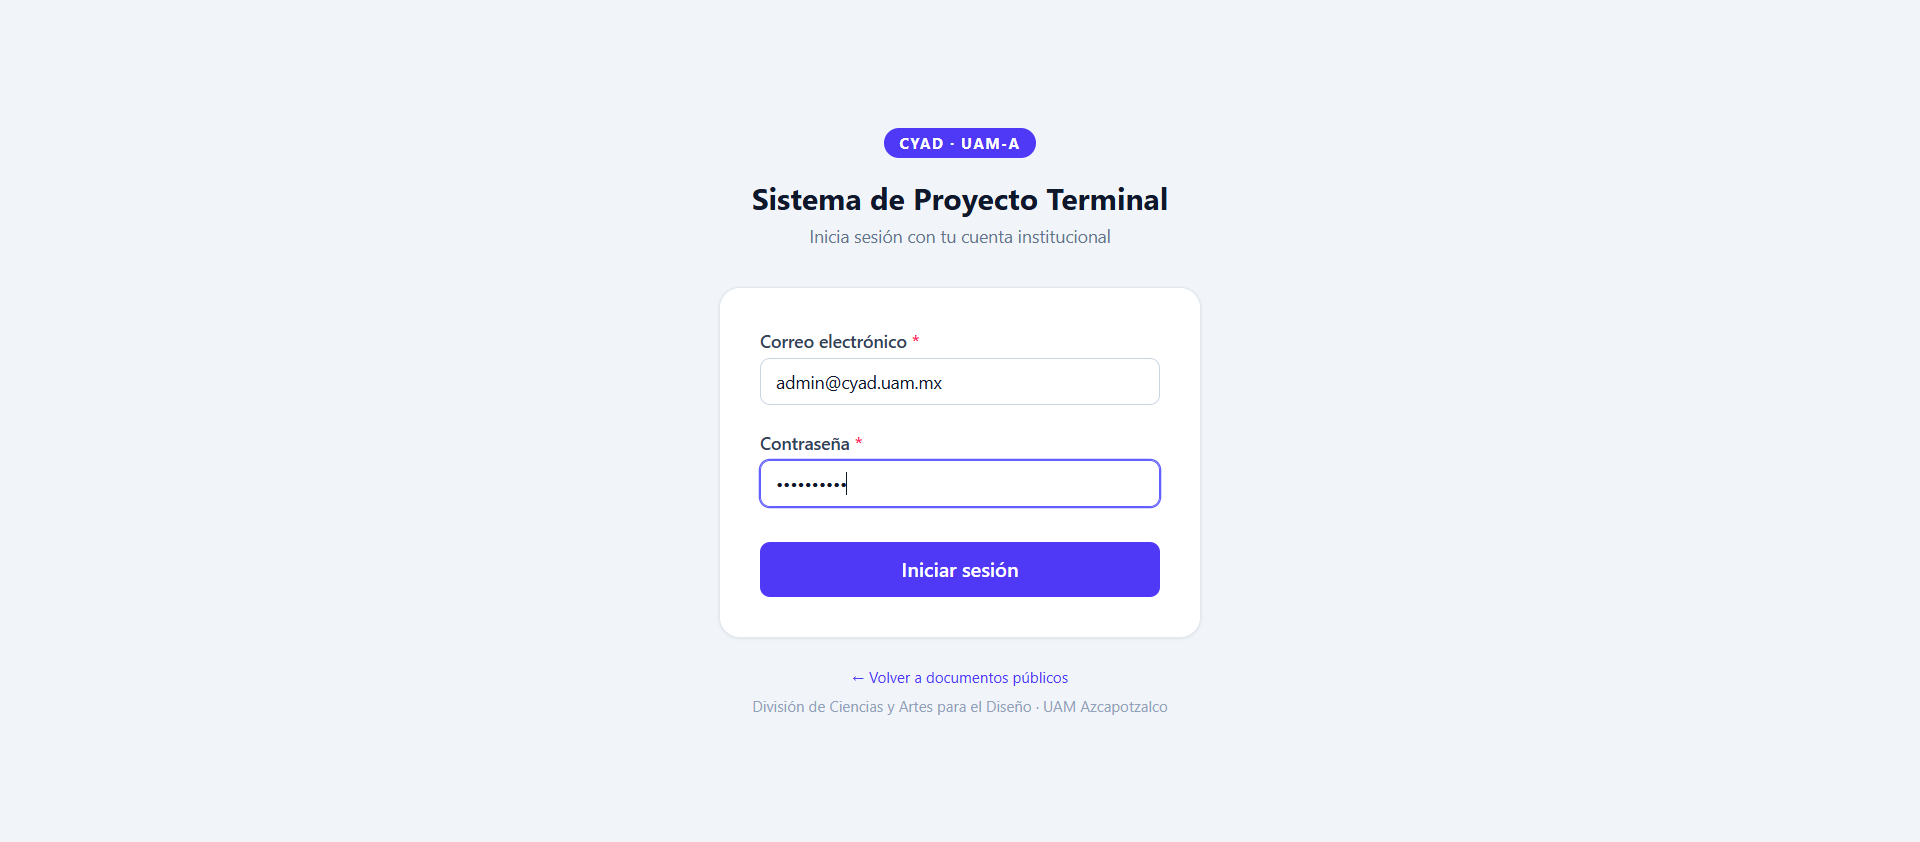
\includegraphics[width=0.65\textwidth]{img/hallazgos/02_login_admin_form.png}
    \caption{Formulario de inicio de sesión (admin).}
\end{figure}

\begin{figure}[H]
    \centering
    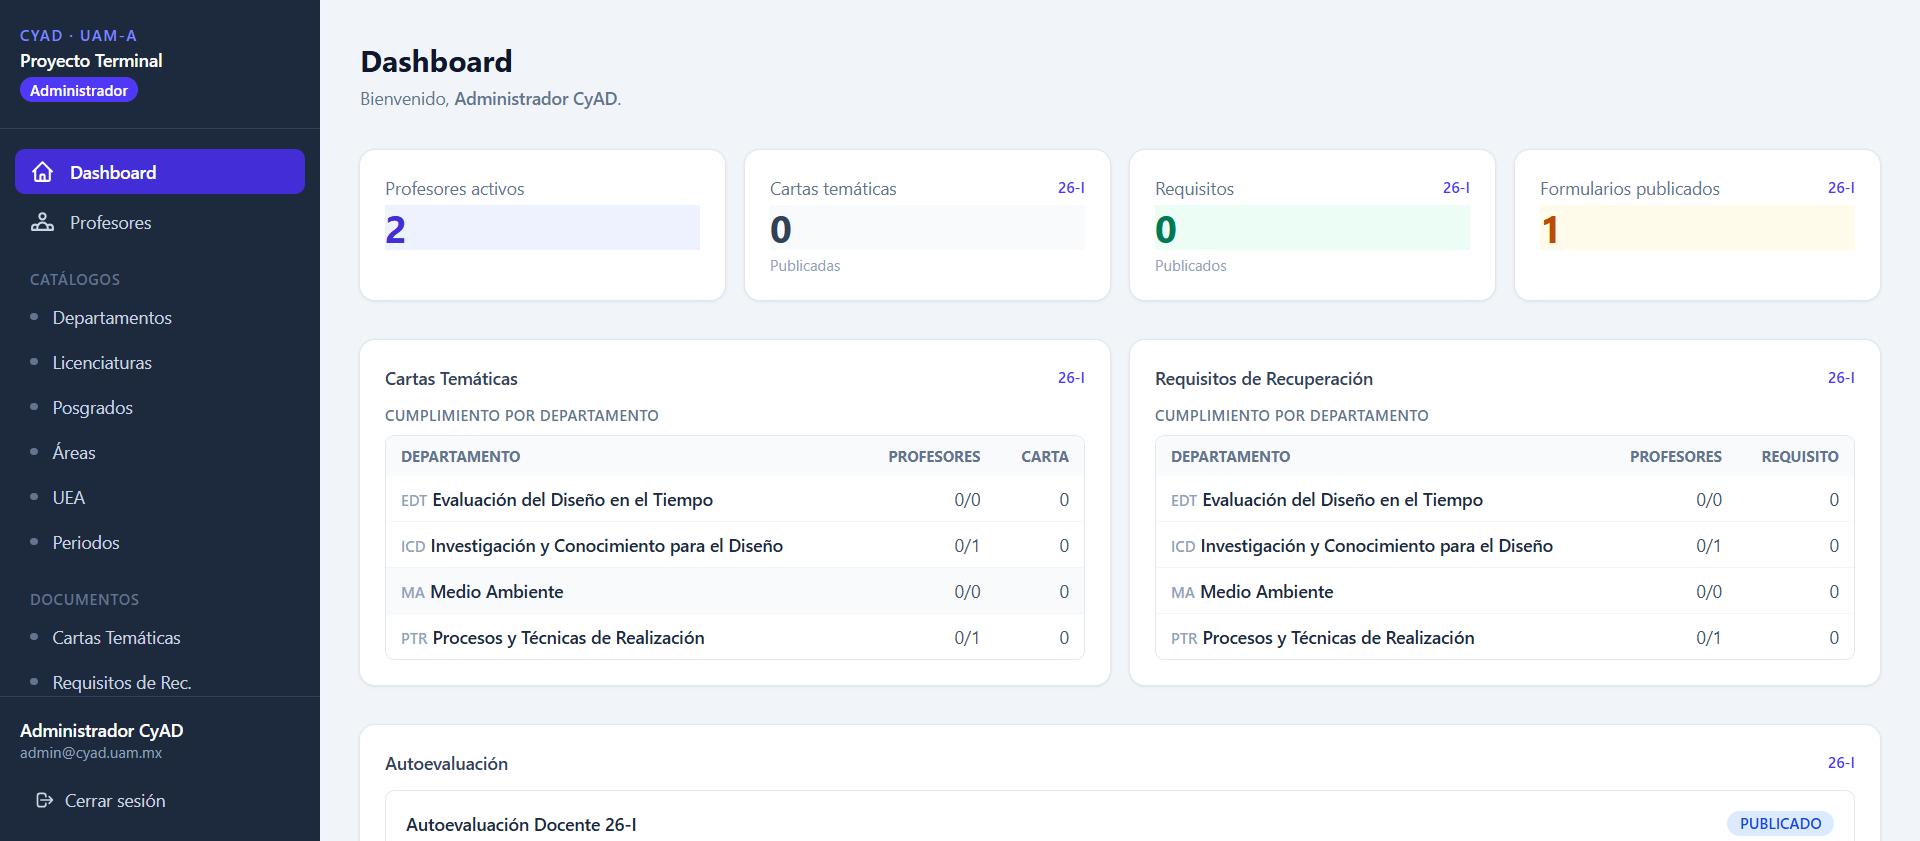
\includegraphics[width=\textwidth]{img/hallazgos/03_dashboard_admin.png}
    \caption{Dashboard del administrador tras iniciar sesión: 2 profesores activos, 1 formulario publicado.}
\end{figure}

\begin{figure}[H]
    \centering
    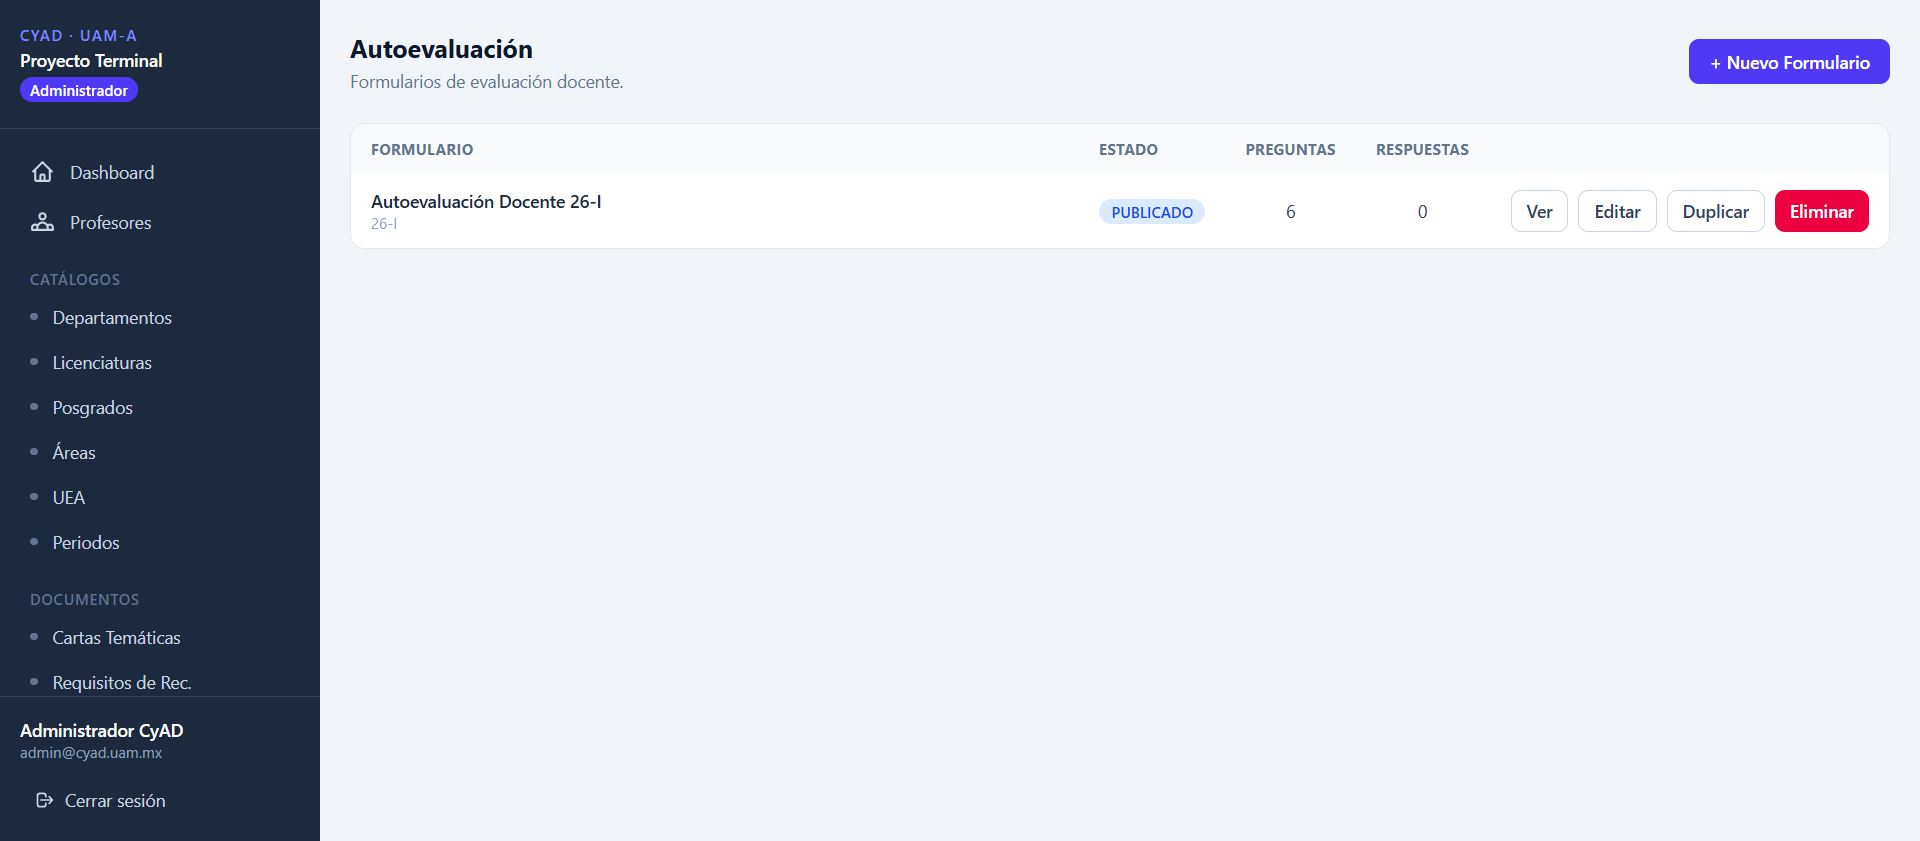
\includegraphics[width=\textwidth]{img/hallazgos/04_admin_autoevaluacion.png}
    \caption{Módulo de Autoevaluación (rol admin) — formulario \emph{Autoevaluación Docente 26-I} en estado \textsc{publicado}, 6 preguntas.}
\end{figure}

\begin{figure}[H]
    \centering
    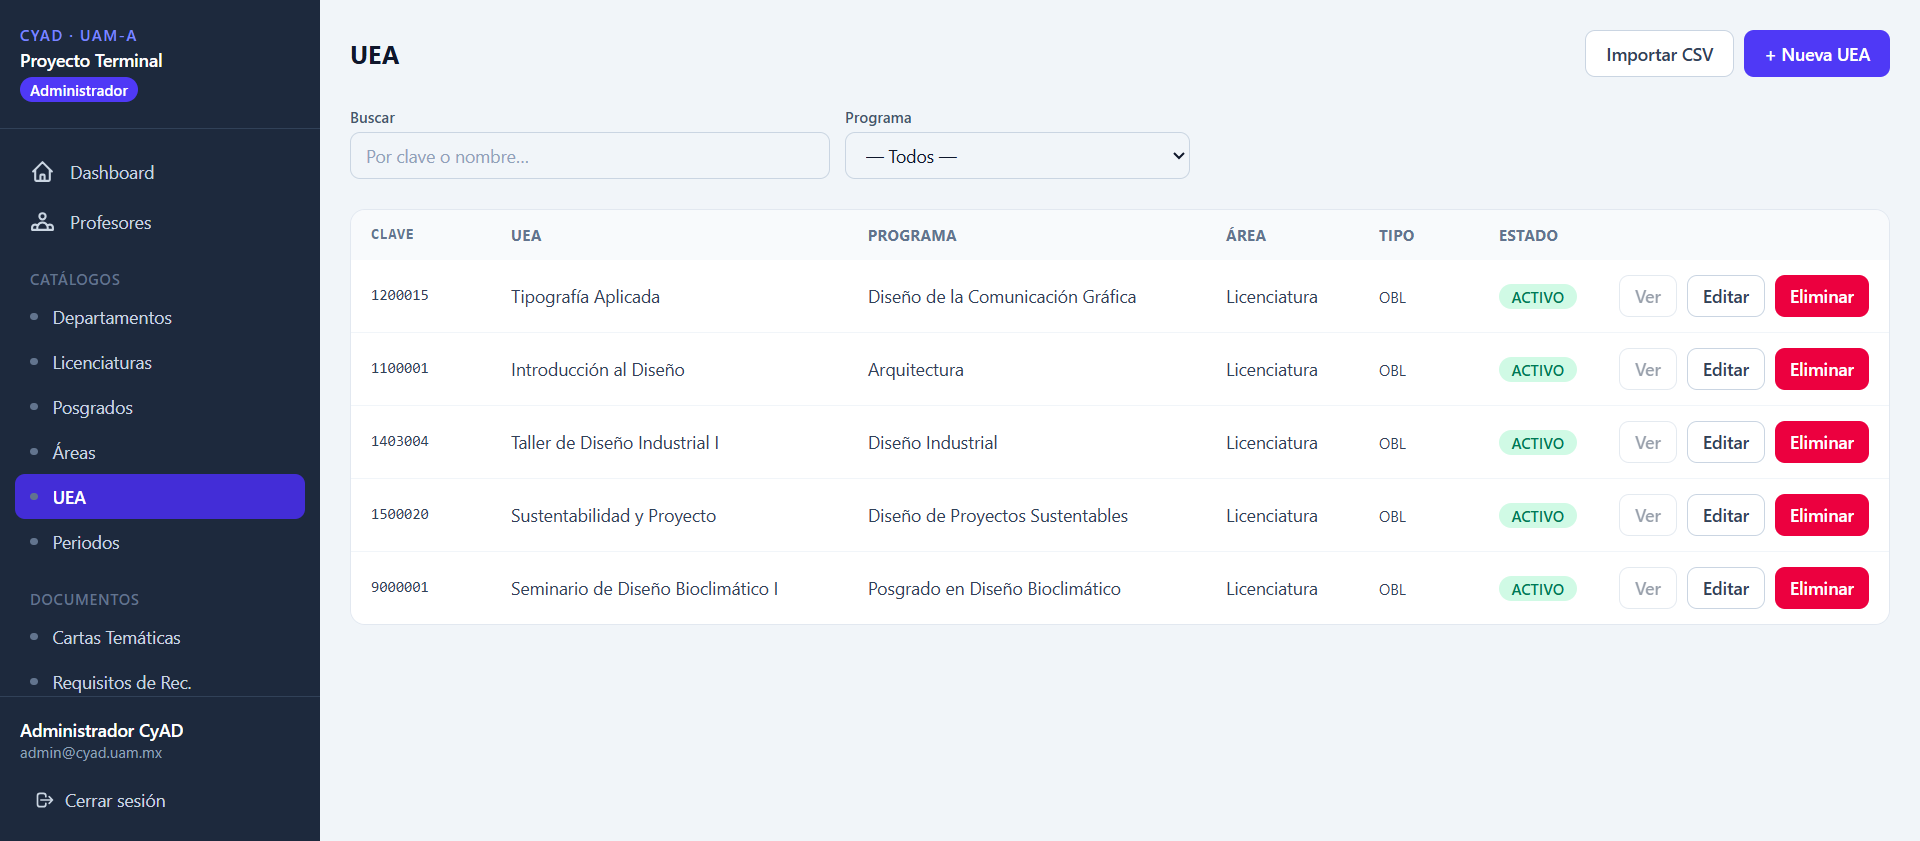
\includegraphics[width=\textwidth]{img/hallazgos/05_admin_uea.png}
    \caption{Catálogo de UEA con las 5 unidades sembradas.}
\end{figure}

\begin{figure}[H]
    \centering
    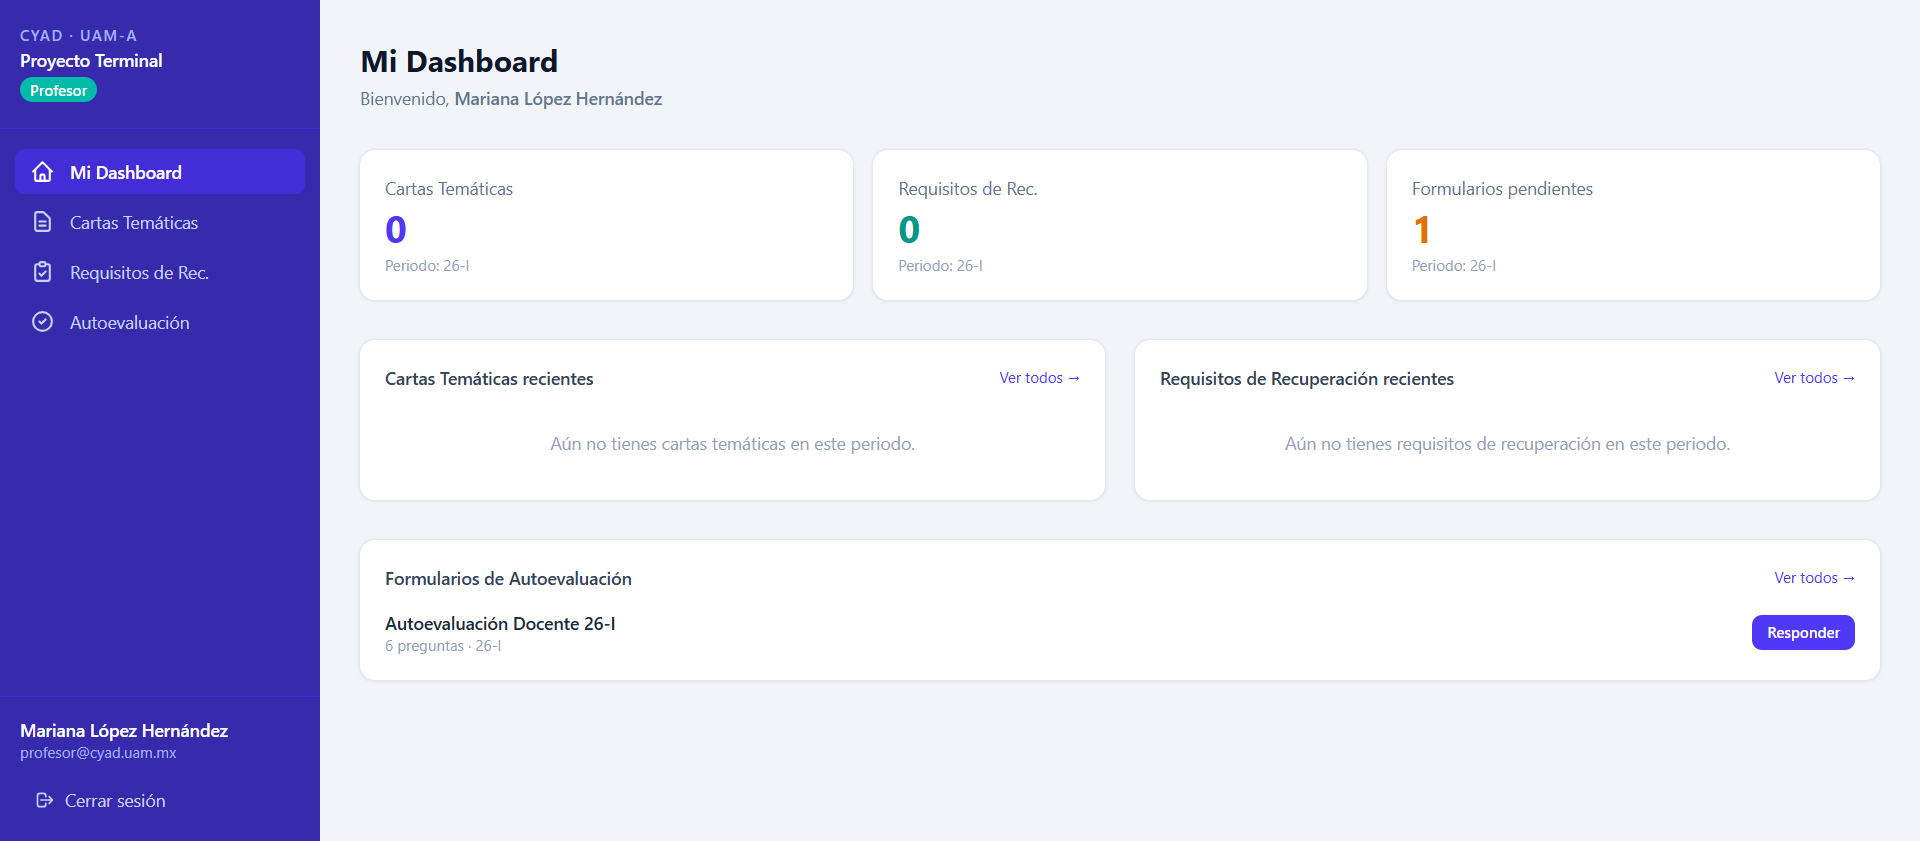
\includegraphics[width=\textwidth]{img/hallazgos/06_dashboard_profesor.png}
    \caption{Dashboard del profesor (Mariana López Hernández) — 1 formulario pendiente correctamente listado.}
\end{figure}

\begin{figure}[H]
    \centering
    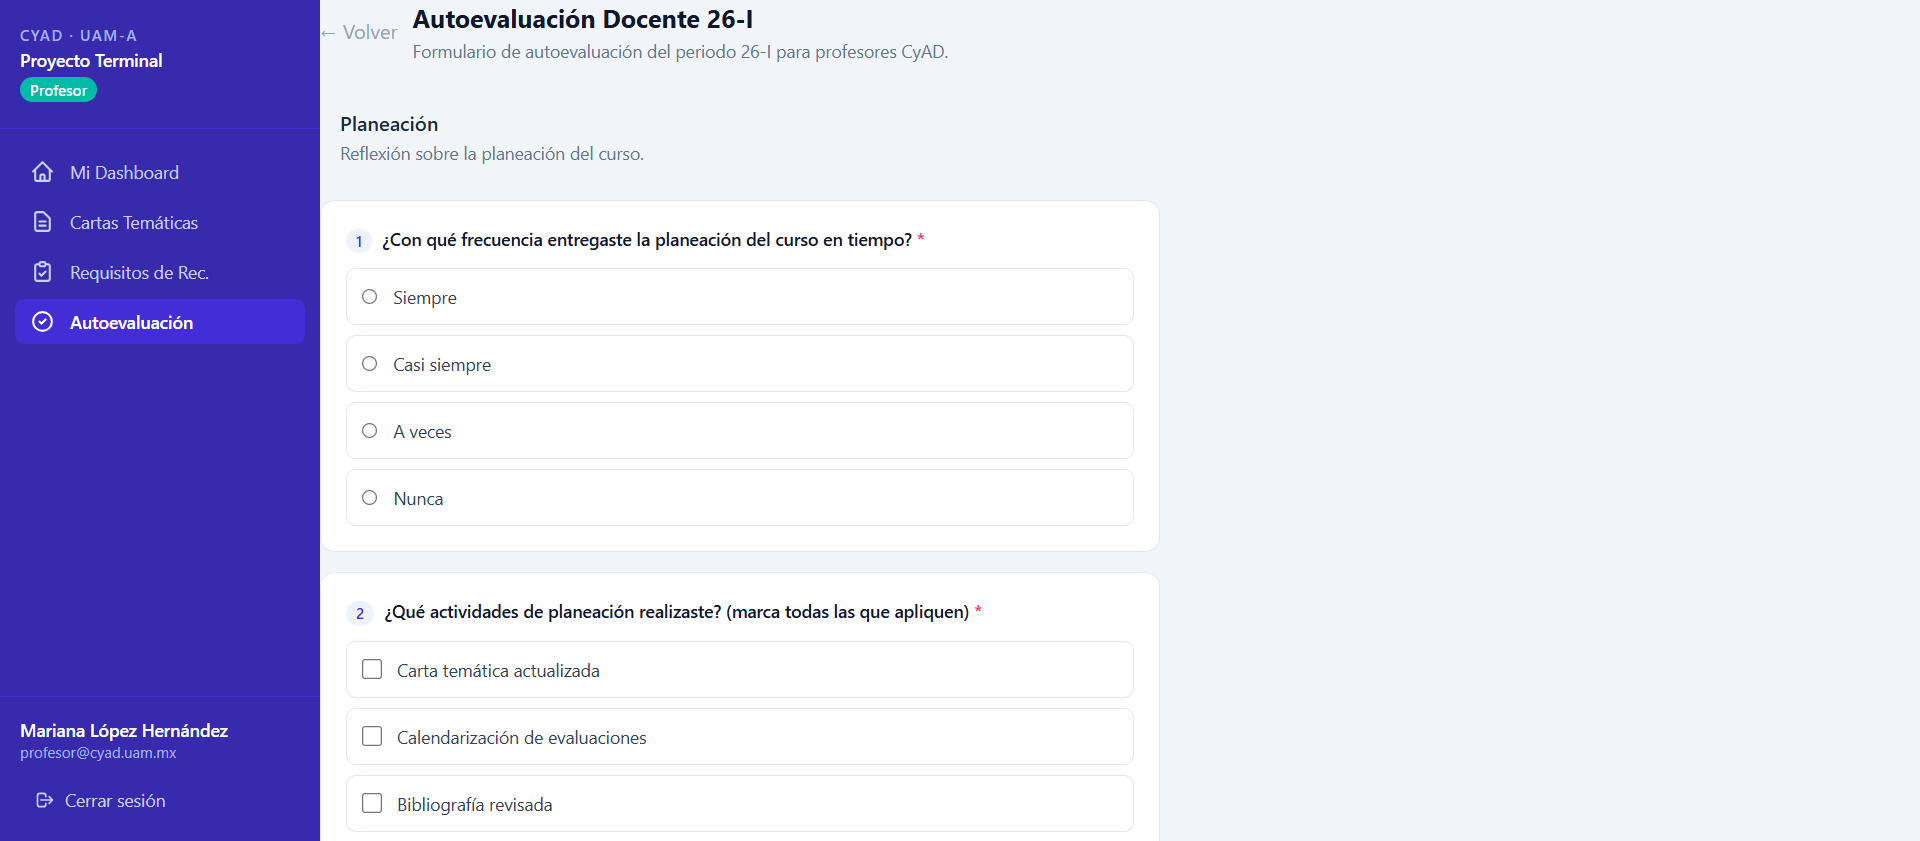
\includegraphics[width=\textwidth]{img/hallazgos/07_profesor_formulario.png}
    \caption{Formulario de autoevaluación listo para responder — dos secciones con pesos 50/50\,\%, 6 preguntas de tipos distintos.}
\end{figure}

Verificación adicional: la consola de DevTools no reporta \emph{errores} ni \emph{warnings} durante la navegación por todas las rutas, incluyendo transiciones entre \emph{chunks} lazy-loaded.

\section{Smoke test}

\begin{Verbatim}[fontsize=\small, frame=single]
$ python scripts/smoke_test.py
=== Salud del backend ===             [OK] GET /health → 200
=== Login ===                         [OK] admin y profesor → 200
=== /auth/me ===                      [OK] rol=ADMIN y rol=PROFESOR
=== Catálogos ===                     [OK] /uea/ (count=5), periodo activo 26-I
=== Autoevaluación — flujo profesor === [OK] formularios-disponibles (count=1),
                                           detalle v1 (6 preguntas),
                                           respuesta id=1
=== Documentos ===                    [OK] POST /cartas-tematicas/ → 201
=== Reportes (admin) ===              [OK] /reportes/dashboard/, cumplimiento

============================================================
SMOKE TEST: TODOS LOS CHECKS OK
real  0m30.541s
\end{Verbatim}

\section{Suite \texttt{pytest} con cobertura}

\begin{Verbatim}[fontsize=\small, frame=single]
$ pytest -q --cov=. --cov-report=term
...
tests/test_auth.py            202   0  100%
tests/test_autoevaluacion.py  932   1   99%
tests/test_catalogos.py       331   0  100%
tests/test_documentos.py      320   2   99%
tests/test_reportes.py        229   0  100%
------------------------------------------
TOTAL                        4411 268   94%
196 passed, 3 warnings in ~400s
\end{Verbatim}

\section{Hallazgos y su resolución}
\label{sec:hallazgos}

Los diez hallazgos originales quedan como sigue tras este ciclo:

\begin{longtable}{p{0.05\textwidth} p{0.34\textwidth} p{0.13\textwidth} p{0.38\textwidth}}
    \toprule
    \textbf{ID} & \textbf{Hallazgo} & \textbf{Estado} & \textbf{Resolución} \\
    \midrule
    \endhead
    H1 & PostgreSQL 16 mínimo indicado por el manual; máquina y README usan 14+/17. & Cerrado (doc) & Manual alineado a ``14+ (probado con 17)''. Commit \texttt{f442c1c}. \\
    \midrule
    H2 & \texttt{psql} no queda en \texttt{PATH} en Windows tras el instalador oficial. & Cerrado (doc) & Nota añadida en prerrequisitos y solución de problemas. Commit \texttt{f442c1c}. \\
    \midrule
    H3 & \texttt{/.env.example} raíz tenía variables JWT obsoletas. & Cerrado (código) & Reemplazadas por \texttt{JWT\_ACCESS\_MINUTES} y \texttt{JWT\_REFRESH\_DAYS}. Commit \texttt{4c2ccc0}. \\
    \midrule
    H4 & \texttt{README.md} instruía \texttt{cp .env.example .env} en la raíz. & Cerrado (código) & Actualizado a \texttt{cd backend \&\& cp .env.example .env}. Commit \texttt{4c2ccc0}. \\
    \midrule
    H5 & \texttt{seed\_demo.py} creaba secciones sin \texttt{peso}. & Cerrado (código) & Añadido \texttt{peso=Decimal("50")} a ambas secciones. Commit \texttt{4c2ccc0}. \\
    \midrule
    H6 & Manual usaba \texttt{VITE\_API\_BASE\_URL} en vez de \texttt{VITE\_API\_URL}. & Cerrado (doc) & Corregido en \texttt{main.tex} sección Frontend. Commit \texttt{f442c1c}. \\
    \midrule
    H7 & 8 vulnerabilidades (1 mod, 7 altas) reportadas por \texttt{npm audit}. & \textbf{Cerrado (código)} & \texttt{npm audit fix} (sin \texttt{--force}) resolvió 7 de 8. La restante (1 alta) es \texttt{xlsx}, \textbf{sin fix upstream disponible}; documentada aquí y en el manual. Commit \texttt{a2b8123}. \\
    \midrule
    H8 & \emph{Bundle} JS de 893 kB (263 kB gzip) tras minificar. & \textbf{Cerrado (código)} & \texttt{React.lazy} + \texttt{Suspense} en las 28 páginas + \texttt{manualChunks} en \texttt{vite.config.js} (separa \texttt{react-vendor}, \texttt{query-vendor}, \texttt{form-vendor} y \texttt{xlsx}). Chunk principal: 893\,kB → 19\,kB (\textbf{{-}98\,\%}). Vite ya no emite warning. Commit \texttt{a2b8123}. \\
    \midrule
    H9 & Discrepancia de versiones mínimas entre manual y README. & Cerrado (doc) & Manual sincronizado con README. Commit \texttt{f442c1c}. \\
    \midrule
    H10 & 4 tests de \texttt{tests/test\_reportes.py} fallaban por la misma causa raíz de H5. & Cerrado (código) & Añadida \texttt{Seccion(peso=100)} antes de cada \texttt{formulario.publicar()} en los 4 tests. 196/196 verde. Commit \texttt{4c2ccc0}. \\
    \bottomrule
\end{longtable}

Todos los hallazgos accionables quedan \textbf{cerrados}. La única vulnerabilidad remanente (\texttt{xlsx}) proviene de una librería sin fix upstream y se acepta como riesgo conocido; alternativas: cambiar a \texttt{exceljs} en un ciclo futuro, o generar los reportes de Excel en el backend con \texttt{openpyxl}.

\section{Bootstrap unificado}

El repositorio incluye ahora \texttt{scripts/bootstrap.ps1} (PowerShell, Windows) que orquesta los tres pasos de preparación de datos en una sola invocación:

\begin{enumerate}
    \item \texttt{python scripts/create\_db.py} — crea la BD en PostgreSQL.
    \item \texttt{python manage.py migrate} — aplica las 38 migraciones.
    \item \texttt{python scripts/seed\_demo.py} — siembra departamentos, licenciaturas, UEAs, profesores demo y el formulario de autoevaluación publicado.
\end{enumerate}

El script asume que el \texttt{.venv} está activo, que las dependencias del backend ya están instaladas (\texttt{pip install -r requirements.txt}), y que \texttt{backend/.env} existe con las credenciales de PostgreSQL. Falla temprano y con mensaje claro si alguno de esos prerrequisitos falta.

Ejecución medida sobre BD limpia: \textbf{9.8 segundos end-to-end}. Sustituye a los tres comandos manuales sin cambiar su semántica; ambos caminos siguen documentados en el manual (sección \emph{Bootstrap unificado} y sección \emph{Datos iniciales}).

\section{Recomendaciones remanentes}

Sólo dos ítems quedan abiertos como mantenimiento futuro (ninguno bloquea la reproducibilidad ni la funcionalidad):

\begin{enumerate}
    \item Sustituir la dependencia \texttt{xlsx} (vulnerabilidad H7 remanente sin fix upstream) por una alternativa mantenida, o generar los reportes de Excel en el backend con \texttt{openpyxl}.
    \item Añadir un equivalente Bash del \emph{bootstrap} (\texttt{scripts/bootstrap.sh}) para usuarios de Linux/macOS. Hoy el manual documenta los tres pasos por separado como alternativa portable.
\end{enumerate}

\section{Veredicto}

El proyecto se monta desde cero, con las siguientes garantías objetivas:

\begin{itemize}
    \item \texttt{scripts/bootstrap.ps1} deja la BD lista en 9.8 segundos, sin intervención manual.
    \item \texttt{npm audit} reporta una única vulnerabilidad remanente (\texttt{xlsx}, sin fix disponible upstream).
    \item \texttt{npm run build} produce 27 \emph{chunks} bien dimensionados; el chunk principal cae de 263 kB gzip a 5 kB gzip.
    \item Las 12 verificaciones del \emph{smoke test} pasan.
    \item La suite \texttt{pytest} pasa \textbf{196/196} con \textbf{94\,\%} de cobertura.
    \item Los flujos de administrador y profesor son navegables sin errores en consola (7 capturas anexas).
\end{itemize}

La reproducibilidad del proyecto está demostrada, ahora también con una experiencia de \emph{one-shot bootstrap} para el mantenedor Windows.

\end{document}
